\documentclass[fontsize=12pt]{book}
\usepackage{tcolorbox}
\usepackage{listings}
\usepackage[usestackEOL]{stackengine}
\usepackage{verbatim}
\usepackage{tikz} 
\usetikzlibrary{arrows,shadows}
\usepackage{pgf-umlsd}
\usepackage{pgf-umlcd}
\usepackage{tikz} 

\newcommand{\insertPython}[1]{ 
\begin{tcolorbox}[title=#1,coltitle=lightgray,width=6in]
\lstinputlisting[language=Python]{../examples/#1}
\end{tcolorbox}
}

\begin{document}
\chapter{What is dīvidere?}

Dīvidere, latin for "to divide, to seperate" seemed an appropriate package name for a distributed system framework project.  
\\
\\
The primary goal of dīvidere is to combine three complementary technologies (Python, ZeroMQ, Protobuf) into a distributed system messaging framework.  ZeroMQ will provide a variety of transport mechanisms, Protobuf providing a language-independent, strongly-typed message encoding and Python the means to combine these components into a reusable framework.

\chapter{ZeroMq}
ZeroMq provides the core transport mechanisms used by this framework.  We'd highhly recommend referencing the official ZeroMq documentation \footnote{Offical ZeroMQ documentation: https://zeromq.org/} for more comprehensive material, but for the purposes of this package we will attempt to document sufficient information necessary to use this package.
\\
The communication package provides primitive ZeroMq classes which support byte-stream messaging as the foundation of other more sophisticated packages.

\section{Publish/Subscribe}
The publish-subscribe, pub-sub, sometimes referred to as the observer pattern is a software design pattern where producers of messages provide info without knowledge of the recepients.  An analogy would be a radio broadcasting station, sending information to an unknown number of recepients.  The messaging is one-way, from provider (publisher) to consumer (subscriber).  A publisher can choose to produce one specific message, or a series of messages.  The subscriber 'subscribes' to a list of messages, afterwhich all produced messages of this 'topic' will be received by the subscriber.
\\
\section{Request/Response}
The request-response, or request-reply, provides a sychronous form of message passing.  The requester sends a message, then waits for the response.  This form of communication enforces a send/receive protocol, failure to comply results in the socket throwing an exception.  You may choose to connect multiple response objects to the same requester, if doing so sent messages will be routed one-by-one to each response objects in a round-robin fashion.  This pattern allows a worker pool fashion architecture.

\chapter{Protobuf}
The ZeroMQ transport supports byte-stream and string payloads.  Complex messages \underline{could} be transmitted in JSON form using the communication package but instead we chose to utilize the protobuf encoding/decoding to allow type-safe, language specific messaging contents.  Google Protobuf \footnote{https://protobuf.dev/} supports a platform-neutral extensible means to define serialing structured data.  Messages are defined in a *.proto file, a message compiler converts the proto file into a language-specific (e.g. Python) message library used by the clients.
\\
\chapter{Architecture}

Dividere is implemented as a layered architeture, the primary communication layer provided at the \emph{Communications} package, the \emph{Messaging} package providing aggregator classes utilizing the communications classes exchanging Protobuf messages.  
\\
These two layers are expected to expand in the future, we also intend on adding higher-level layer(s) with higher-level distributed system abstractions.
\\

  {
     \vbox {
        \framebox[6in]{\stackunder{ \large{Service} }{
            \fbox{\stackunder{ ServiceRegistry.Server }{}}  
            \fbox{\stackunder{ ServiceRegistry.Client }{}}  
            \fbox{\stackunder{ Service }{}}  
            }}  
      }
     \vbox {
        \framebox[6in]{\stackunder{ \large{Messaging} }{
            \fbox{\stackunder{ Publisher }{}}  
            \fbox{\stackunder{ Subscriber }{}}  
            \fbox{\stackunder{ Request }{}}  
            \fbox{\stackunder{ Response }{}}  
            \fbox{\stackunder{ Dealer }{}}  
            \fbox{\stackunder{ MsgReactor }{}}  
            }}  
      }
      \vbox {
        \framebox[6in]{\stackunder{ \large{Communications} }{
            \fbox{\stackunder{ Connector }{}}  
            \fbox{\stackunder{ Publisher }{}}  
            \fbox{\stackunder{ Subscriber }{}}  
            \fbox{\stackunder{ Request }{}}  
            \fbox{\stackunder{ Response }{}}  
            \fbox{\stackunder{ Proxy }{}}  
            \fbox{\stackunder{ Dealer }{}}  
            }}  
      }
 } 

Dividere implements a layered architecture approach, more primitive abstractions located at the lower layers, with specialized abstractions atop.  Upper layers utilizing lower layer componenents.

\section{Communications}
The communications layer focuses on providing string-based messaging components with generalized debugging visibility.  Each consumer component allows blocking and time-out blocking message retrieval interfaces.  Most of these components provide a light-weight facade to ZeroMQ components.

\section{Messaging}
This layer mirrors many of the components from the communications layer with a subtle difference, components in this layer utilize protobuf messaging protocol rather than string-based messages.  This layer is intended to provide multi-language integration support.

\section{Service}
The service layer provides service-based abstactions, including a 'Service' abstract class that registers with the centralized, server-based, name-service.

\chapter{Class Design}


%\begin{sequencediagram}
%    \newinst{act}{Actor}
%    \newthread{nr}{NetRoute}
%    \newthread{nr}{NetScan}
%    \begin{call}{act}{ Buscar una red}{nr}{ redes }
%        %\begin{call}{act}{ Buscar una red}{nr}{ redes }
%    \end{call}
%\end{sequencediagram}

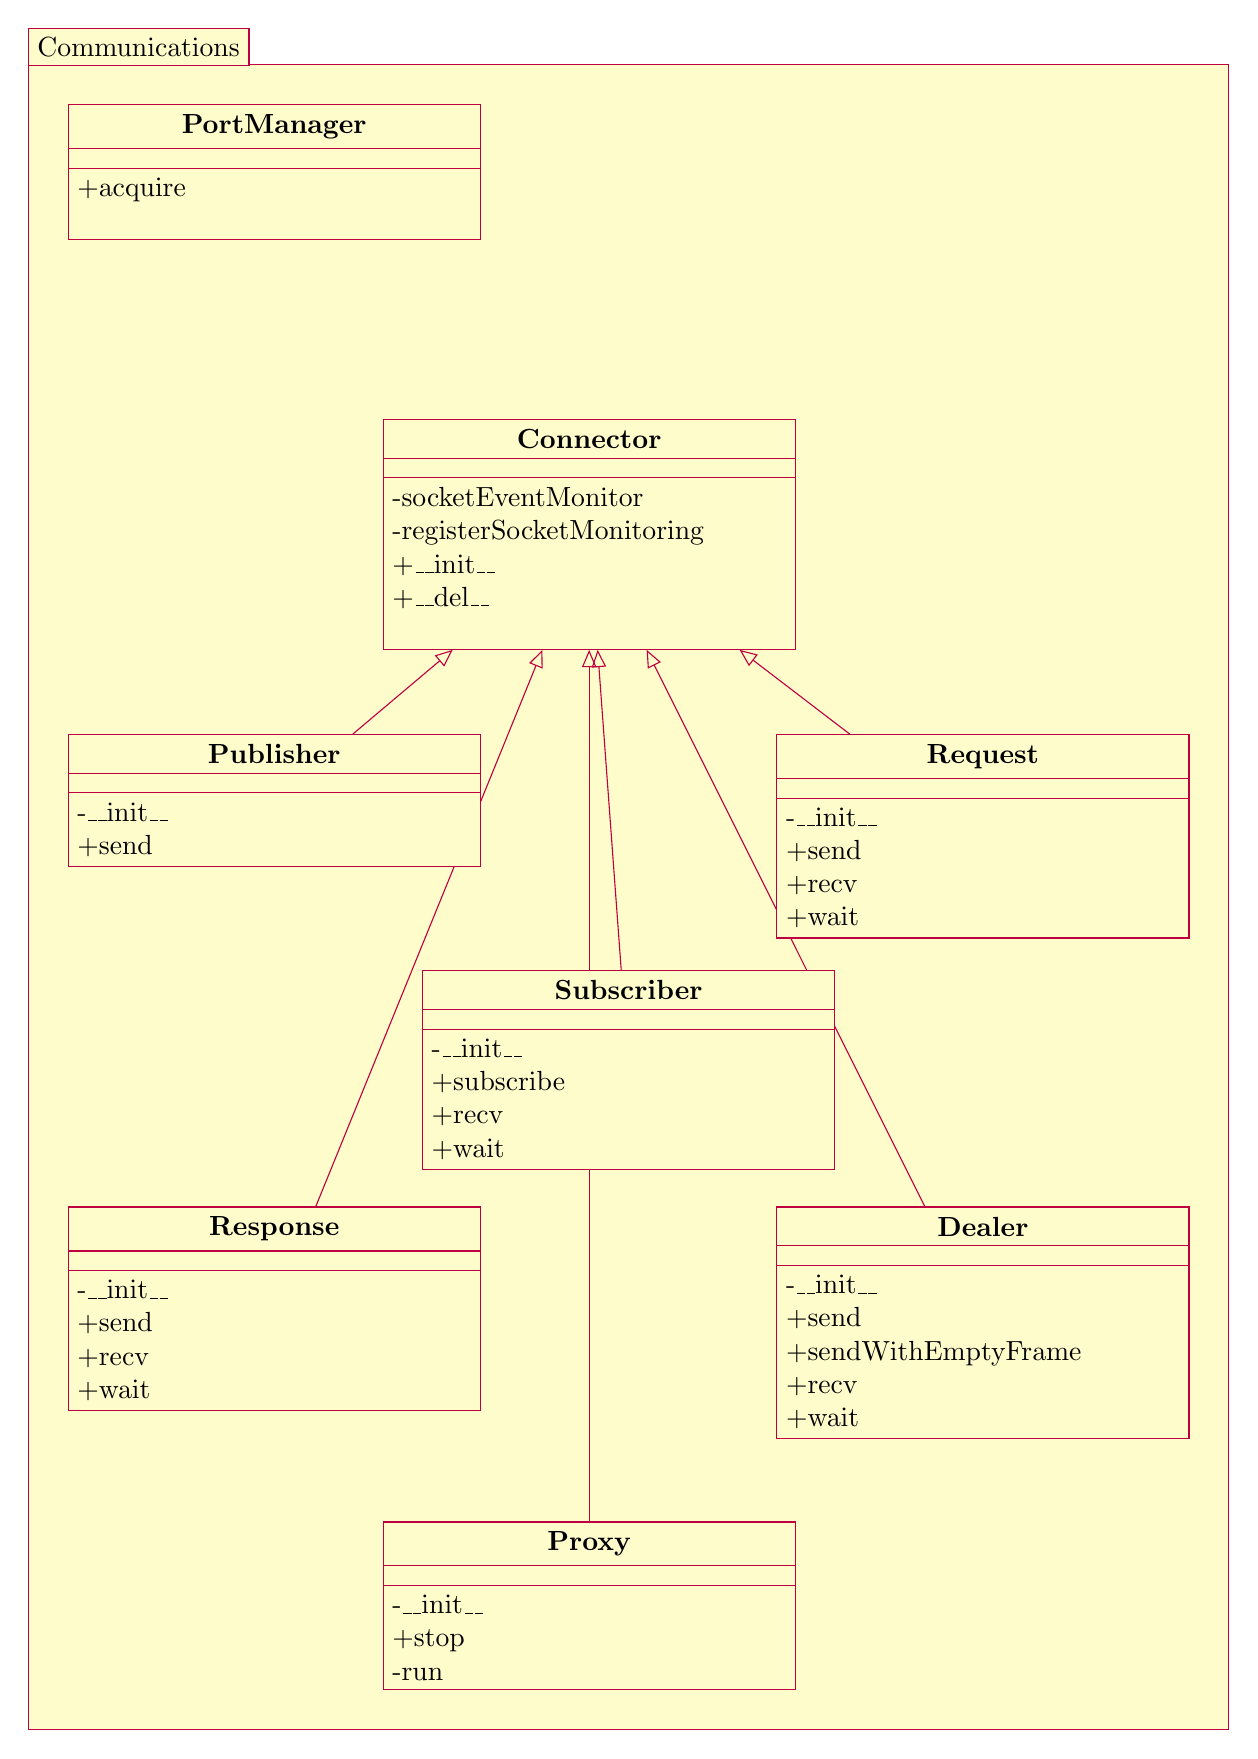
\begin{tikzpicture}
  \begin{package}{Communications}
    \begin{class}{PortManager}{0,8}
      \operation{+acquire}
      \operation{}
    \end{class}
  
    \begin{class}{Connector}{4,4}
      \operation{-socketEventMonitor}
      \operation{-registerSocketMonitoring}
      \operation{+\_\_init\_\_}
      \operation{+\_\_del\_\_}
      \operation{}
    \end{class}
  
    \begin{class}{Publisher}{0,0}
      \inherit{Connector}
      \operation{-\_\_init\_\_}
      \operation{+send}
    \end{class}
  
    \begin{class}{Subscriber}{4.5,-3}
      \inherit{Connector}
      \operation{-\_\_init\_\_}
      \operation{+subscribe}
      \operation{+recv}
      \operation{+wait}
    \end{class}
  
    \begin{class}{Request}{9,0}
      \inherit{Connector}
      \operation{-\_\_init\_\_}
      \operation{+send}
      \operation{+recv}
      \operation{+wait}
    \end{class}
  
    \begin{class}{Response}{0,-6}
      \inherit{Connector}
      \operation{-\_\_init\_\_}
      \operation{+send}
      \operation{+recv}
      \operation{+wait}
    \end{class}
  
    \begin{class}{Dealer}{9,-6}
      \inherit{Connector}
      \operation{-\_\_init\_\_}
      \operation{+send}
      \operation{+sendWithEmptyFrame}
      \operation{+recv}
      \operation{+wait}
    \end{class}
  
    \begin{class}{Proxy}{4,-10}
      \inherit{Connector}
      \operation{-\_\_init\_\_}
      \operation{+stop}
      \operation{-run}
    \end{class}
  \end{package}

\end{tikzpicture}

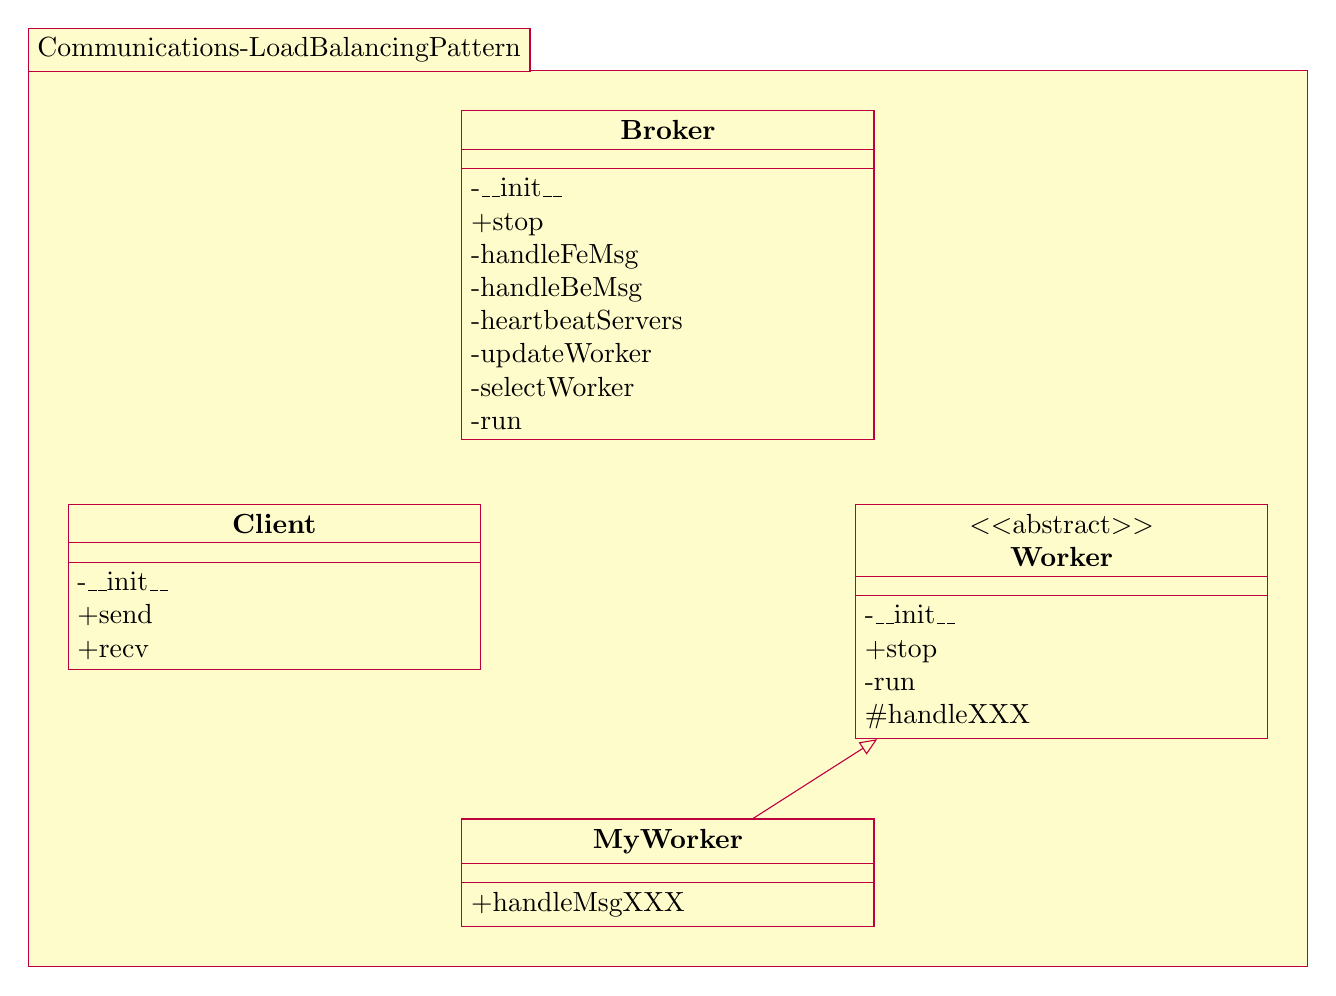
\begin{tikzpicture}
  \begin{package}{Communications-LoadBalancingPattern}
    \begin{class}{Broker}{0,0}
      \operation{-\_\_init\_\_}
      \operation{+stop}
      \operation{-handleFeMsg}
      \operation{-handleBeMsg}
      \operation{-heartbeatServers}
      \operation{-updateWorker}
      \operation{-selectWorker}
      \operation{-run}
    \end{class}
    \begin{abstractclass}{Worker}{5,-5}
      \operation{-\_\_init\_\_}
      \operation{+stop}
      \operation{-run}
      \operation{\#handleXXX}
    \end{abstractclass}
    \begin{class}{Client}{-5,-5}
      \operation{-\_\_init\_\_}
      \operation{+send}
      \operation{+recv}
    \end{class}
    \begin{class}{MyWorker}{0,-9}
      \inherit{Worker}
        \operation{+handleMsgXXX}
    \end{class}
  \end{package}
\end{tikzpicture}
\\
\\
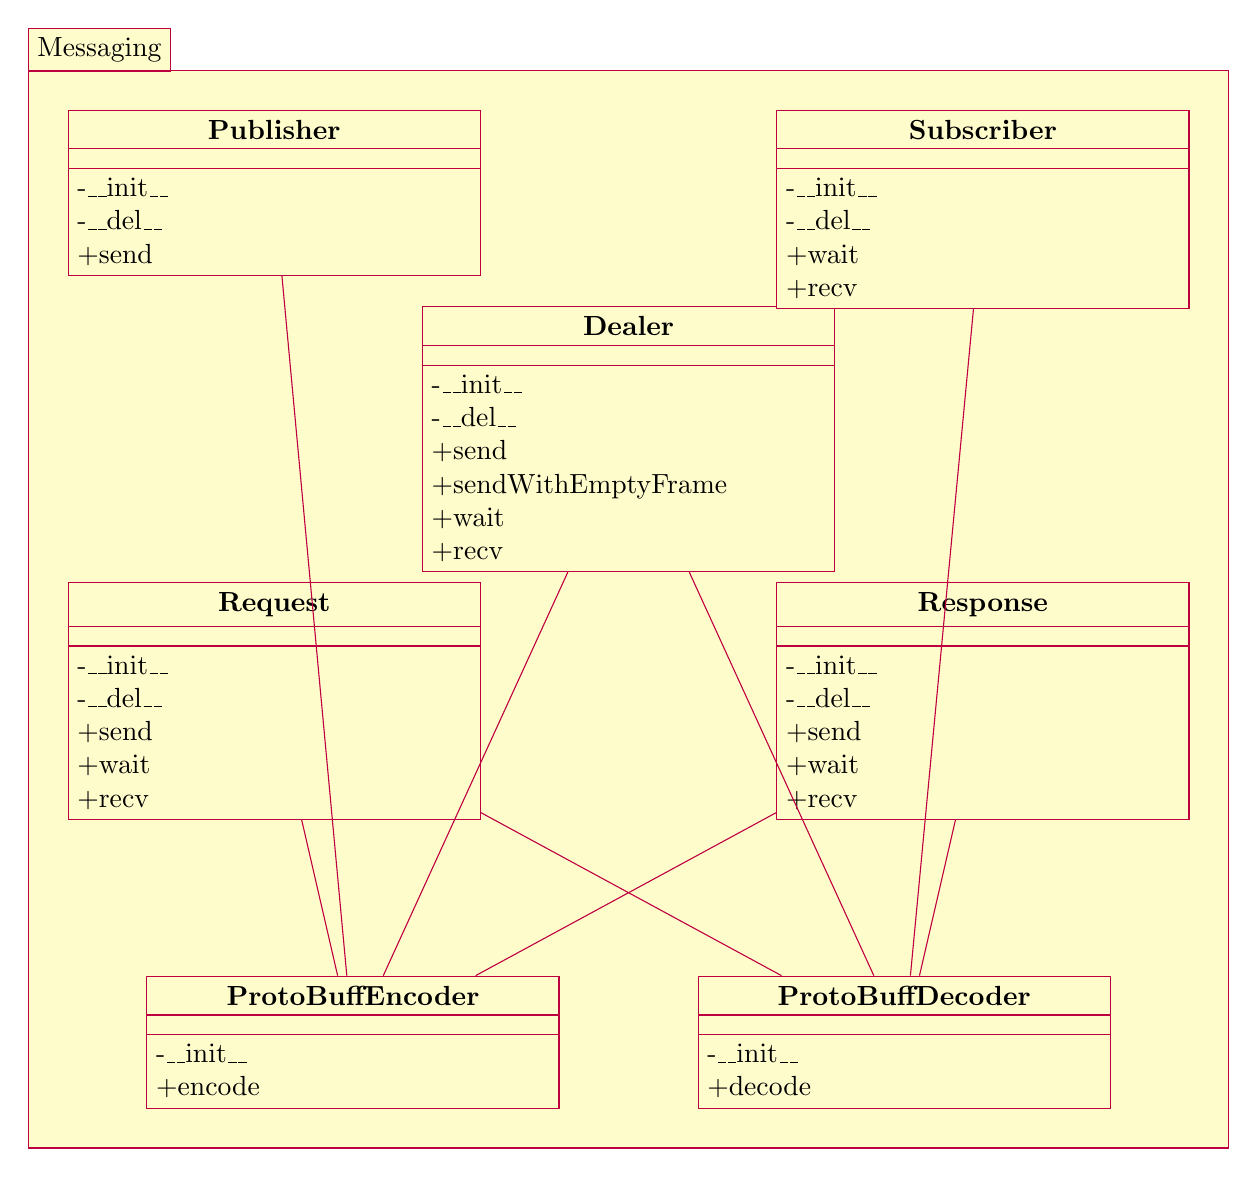
\begin{tikzpicture}
  \begin{package}{Messaging}
    \begin{class}{Request}{0,0}
      \operation{-\_\_init\_\_}
      \operation{-\_\_del\_\_}
      \operation{+send}
      \operation{+wait}
      \operation{+recv}
    \end{class}
    \begin{class}{Response}{9,0}
      \operation{-\_\_init\_\_}
      \operation{-\_\_del\_\_}
      \operation{+send}
      \operation{+wait}
      \operation{+recv}
    \end{class}
    \begin{class}{Dealer}{4.5,3.5}
      \operation{-\_\_init\_\_}
      \operation{-\_\_del\_\_}
      \operation{+send}
      \operation{+sendWithEmptyFrame}
      \operation{+wait}
      \operation{+recv}
    \end{class}
    \begin{class}{Publisher}{0,6}
      \operation{-\_\_init\_\_}
      \operation{-\_\_del\_\_}
      \operation{+send}
    \end{class}
    \begin{class}{Subscriber}{9,6}
      \operation{-\_\_init\_\_}
      \operation{-\_\_del\_\_}
      \operation{+wait}
      \operation{+recv}
    \end{class}

    \begin{class}{ProtoBuffEncoder}{1,-5}
      \operation{-\_\_init\_\_}
      \operation{+encode}
    \end{class}
    \begin{class}{ProtoBuffDecoder}{8,-5}
      \operation{-\_\_init\_\_}
      \operation{+decode}
    \end{class}

    \association {Subscriber}{}{}{ProtoBuffDecoder}{}{}
    \association {Publisher}{}{}{ProtoBuffEncoder}{}{}
    \association {Dealer}{}{}{ProtoBuffEncoder}{}{}
    \association {Dealer}{}{}{ProtoBuffDecoder}{}{}
    \association {Request}{}{}{ProtoBuffEncoder}{}{}
    \association {Request}{}{}{ProtoBuffDecoder}{}{}
    \association {Response}{}{}{ProtoBuffEncoder}{}{}
    \association {Response}{}{}{ProtoBuffDecoder}{}{}
  \end{package}
\end{tikzpicture}
\\
\\
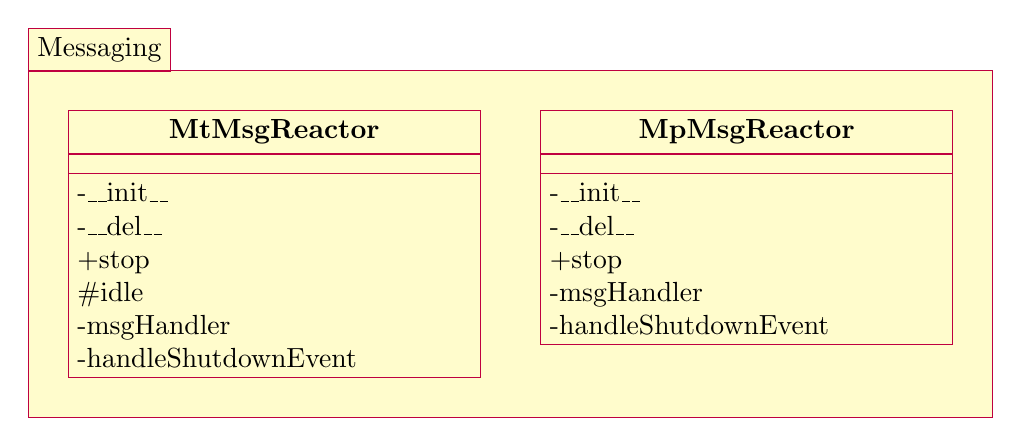
\begin{tikzpicture}
  \begin{package}{Messaging}
    \begin{class}{MtMsgReactor}{-3,0}
      \operation{-\_\_init\_\_}
      \operation{-\_\_del\_\_}
      \operation{+stop}
      \operation{\#idle}
      \operation{-msgHandler}
      \operation{-handleShutdownEvent}
    \end{class}
    \begin{class}{MpMsgReactor}{3,0}
      \operation{-\_\_init\_\_}
      \operation{-\_\_del\_\_}
      \operation{+stop}
      \operation{-msgHandler}
      \operation{-handleShutdownEvent}
    \end{class}
  \end{package}
\end{tikzpicture}
\\
\\
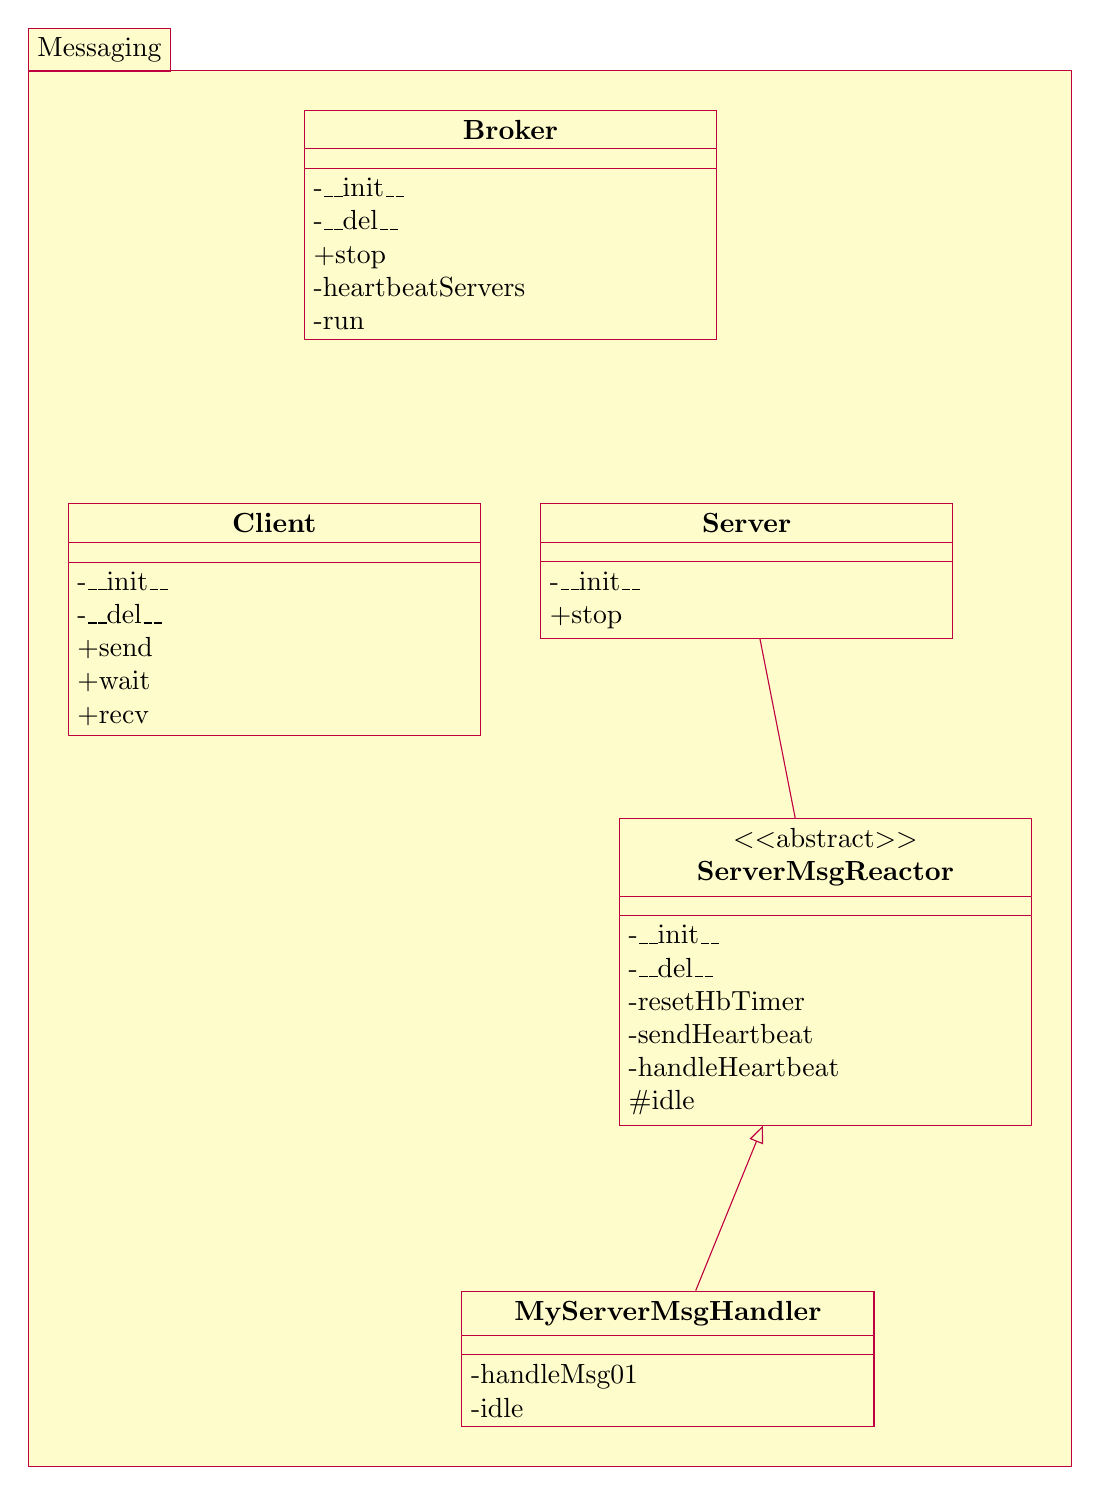
\begin{tikzpicture}
  \begin{package}{Messaging}
    \begin{class}{Broker}{0,0}
      \operation{-\_\_init\_\_}
      \operation{-\_\_del\_\_}
      \operation{+stop}
      \operation{-heartbeatServers}
      \operation{-run}
    \end{class}
    \begin{class}{Client}{-3,-5}
      \operation{-\_\_init\_\_}
      \operation{-\_\_del\_\_}
      \operation{+send}
      \operation{+wait}
      \operation{+recv}
    \end{class}
    \begin{class}{Server}{3,-5}
      \operation{-\_\_init\_\_}
      \operation{+stop}
    \end{class}
    \begin{abstractclass}{ServerMsgReactor}{4,-9}
      \operation{-\_\_init\_\_}
      \operation{-\_\_del\_\_}
      \operation{-resetHbTimer}
      \operation{-sendHeartbeat}
      \operation{-handleHeartbeat}
      \operation{\#idle}
    \end{abstractclass}
    \association {Server}{}{}{ServerMsgReactor}{}{}

    \begin{class}{MyServerMsgHandler}{2,-15}
      \inherit{ServerMsgReactor}
      \operation{-handleMsg01}
      \operation{-idle}
    \end{class}
  \end{package}
\end{tikzpicture}

\chapter{Examples}
\insertPython{simplePubSub.py}
\insertPython{msgReactor.py}

\chapter{Reference}
\verbatiminput{ref.txt}
\end{document}
